\subsection{Formato}
El punto clave para que el usuario entienda lo que queremos transmitirle es crear una comunicacion fluida entre la representacion
de los datos el usuario. Para ello  deberemos asegurarnos que hablamos el mismo idioma, con un vocabulario facil de entender y
con proximidad, es decir,dejar la terminologia a un lado y comunicar el objetivo de la manera mas simple posible.
Por ello la representacion de la informacion jugaran un papel fundamental para que la 
informacion sea absorbida por el usuario de una manera natural.


\subsubsection{How to solve it} 
Este modelo debera proporcionar la informacion al usario en un lenguaje o formato compresible. Si no es posible proporcionaremos las 
herramientas necesarias para que este pueda comprender el contexto de la informacion.
Deberemos estudiar que tipo de representacion es mas adecuada, no siempre una grafica es la representacion mas adecuada, deberemos hacer un 
estudio de tanto al publico al que va dirigido como como podemos acentuar la informacion que sea mas relevante en la manera 
correcta.
Si nos declinamos por realizar una representacion con graficas, deberemos estudiar los datos para saber que tipo de grafica. Por ejemplo, 
si hablamos de muestras y queremos saber la densidad, nos inclinaremos por un grafico de densidad y si por ejemplo buscamos la diferencia 
entre sexos, utilizaremos un grafico de tartas.

\subsubsection{How we solve it. Aire Guru} 
La herramienta Aire guru presenta la informacion en el idioma nativo de la ciudad y se utiliza un lenguaje sencillo y directo.
Se utilizan colores y recursos graficos como iconos. Ademas se ha elegido una estructura para representar los datos y se repite en disdintas 
partes en vez de crear una visualizacion distinta, asi el usuario solo debe asimilar una unica formula.

Unos de los objetivos es representa la contaminacion por zonas de la ciudad, por lo que se ha utilizado un mapa sobre el que se representa
 el AQI general calculado. Este es un formato mas legible para los usuarios ya que no tiene que trabajar para realizar una imagen visual
 de los distintos lugares de la ciudad. Este indice mustra un indicador con cinco niveles representados por una escala de colores desde el 
 turquesa hasta el rojo ("Bueno" "Aceptable""Pobre" "Malo" e "Insalubre"). La razon de esta eleccion es porqu eson los colores oficiales y 
 asi se evita crear confusion al usuario si consulta las fuentes oficiales.
 \newpage
 \begin{figure}[ht]
    \centering
    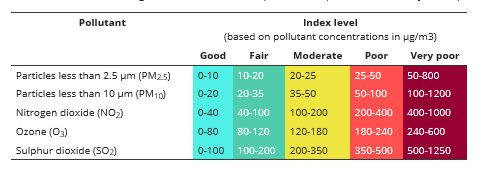
\includegraphics[width=12cm]{EAQI}
    \caption{EAQI Levels}
\end{figure}

La iconografica utilizada para ayudar al usuario a tener una idea directa de la situacion, ya que son mas 
explicativos que los colores. En caso de peligro, queda bien representado con el color rojo, pero en el caso del azul o verde, en nuestra cultura, no
tenemos definido un estado para estos colores.\\
\begin{figure}[ht]
    \centering
    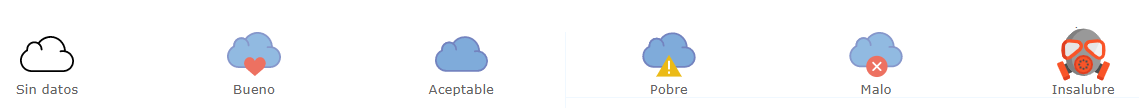
\includegraphics[width=10cm]{EAQI_Icons}
    \caption{Iconografica Aire Guru}
\end{figure}

Para las graficas que muestran variaciones en el tiempo, se han utilizado graficos de lineas, que son las mas apropiadas para este tipo de datos,
ya que muestran la continua evolucion durante un periodo de tiempo. Para representar los distintos componentes del AQI se ha utilizado un
grafico de barras apiladas, ya que se ve que proporcion del AQI total esta formada por que contaminante.\\
\begin{figure}[ht]
    \centering
    \subfigure[AQI Evolution]
     {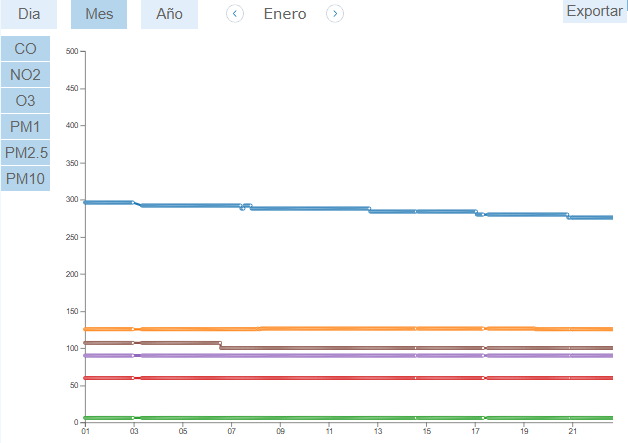
\includegraphics[width=5.75cm]{lineChart}}
     \hfill
     \subfigure [AQI components]
    { 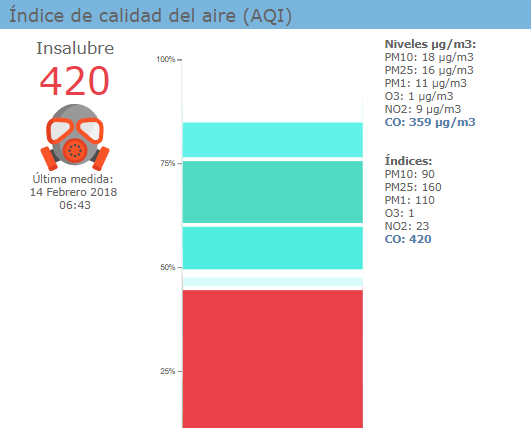
\includegraphics[width=5.25cm]{stakedBarChart}}
 
    \caption{Charts}
\end{figure}

Ademas, para explicar el concepto de AQI y crear un awarnes sobre la influencia que tiene en nosotros la polucion del aire, Aire Guru proporciona un 
glosario y una ayuda con las descripciones de los agentes contaminantes, complicaciones medicas, fuentes de contaminacion, la iconografia utilizada y
una explicacion sobre que es y como se calcula el AQI.\\

 
\elsparagraph{Evaluation}  
\begin{itemize}
    \done El lenguaje utilizado en toda la herramienta es un lenguaje comun, huye de la terminologia cientifica pero proporciona la informacion
    suficiente para enteder la situacion.
    \done Se han estudiado y utilizado las graficas mas apropiadas para cada tipo de datos.
    \crossed Algunos terminos especificos no se han podido sustituir como "Indice de calidad del Aire".
    \done Se han proporcionado la herramientas necesarias para entender el concepto. Se ha utilizado la norma europea de calidad del aire para 
    representar los valores y se ofrece al usuario recursos en la pagina para su comprension ademas de recursos extenos.
    
\end{itemize}
 

\newpage